\documentclass[12pt, titlepage]{article}
\usepackage{graphicx}
\usepackage{amsmath}
\usepackage{tcolorbox}
\usepackage{parskip}
\usepackage[]{fancyhdr}
\usepackage{pgfplots}
\pgfplotsset{compat=1.18}
\setlength{\headheight}{15pt}
\tcbuselibrary{breakable}

\title{Electric Potential}
\author{Matthew Pan}
\date{February 2025}

\newtcolorbox{Problem}{colback=blue!5!white,colframe=blue!50!black,title=Problem, breakable=true}

\begin{document}

\pagestyle{fancy}

\fancyhead{}
\fancyhead[L]{Pan}
\fancyhead[R]{\thepage}

\maketitle

\section*{Topic 9.1 - Electric Potential Energy}
It's often helpful to compare electrostatic terms with similar gravitational terms

Comparing electric potential energy and gravitational potential energy:
\begin{itemize}
    \item{Both require two objects in a system}
    \item{Both are proportional to $\frac{1}{r}$}
\end{itemize}

\begin{center}
\begin{tabular}{ c c }
    $U_E=\frac{kq_1q_2}{r}$ & $U_G=\frac{Gm_1m_2}{r}$
\end{tabular}
\end{center}

\begin{Problem}
    Calculate the electric potential energy of two point charges placed 1.5cm apart. Charge 1 has a charge of +4 C and charge 2 has a charge of +6 C.
    \\ \\
    How does the answer change if charge 2 is -6C? 

    \tcblower

    \textit{Solution. \\}
    a)
    \begin{equation*}
    \begin{split}
            U_E&=\frac{9 \times 10^9 \cdot +4 \cdot +6}{0.015} \\
            &=1.44 \times 10^{13} J
    \end{split}
    \end{equation*}

    b)
    \begin{equation*}
        \begin{split}
                U_E&=\frac{9 \times 10^9 \cdot +4 \cdot -6}{0.015} \\
                &=-1.44 \times 10^{13} J
        \end{split}
        \end{equation*}
\end{Problem}

What does it mean for $U_E$ to be negative? \\
Work must be done against the field to move the charged objects away from each other. For example, when a positive and negative point charge are attracted to each other, work must be done to move the charged particles away from each other.

To calculate $U_E$ when three or more charged particles are present, calculate $U_E$ for each pair of objects and sum them. 

\section*{Topic 9.2 - Electric Potential}
\subsection*{Electric Potential and Electric Potential Energy}
Electric potential (V) describes the electric potential energy ($U_E$) per unit charge (q) at a point in space. To help us understand this idea conceptually, we can again refer to a similar concept in gravitation. Let's say that a 1kg ball is on top of a building 10m high. The potential energy $ U_g = mgh$ would be $1 \cdot 9.8 \cdot 10$. So, for every additional kilogram of mass, our potential energy would increase by 98 J. In electrostatics, for every additional coulomb of charge, the potential energy would increase by V. Therefore,
\begin{equation*}
    U_E = qV
\end{equation*}
\begin{equation*}
    V = \frac{U_E}{q} = \frac{kq}{r}
\end{equation*}

\begin{Problem}
    What is the electric potential at a point 5 cm away from a 1$\mu C$ charge? What is $U_E$ if a 1 $\mu C$ charge was placed there? A 2 $\mu C$ charge?

    \tcblower
    \textit{Solution. \\}
    a)
    \begin{equation*}
        \begin{split}
        V&=\frac{kq}{r} \\
        &=\frac{(9 \times 10^{9})(1 \times 10^{-6})}{0.05} \\
        &=1.8 \times 10^{5}
        \end{split}
    \end{equation*}
    b)
    \begin{equation*}
        \begin{split}
        U_E &= qV \\
        &= (1 \times 10^{-6})(1.8 \times 10^{5}) \\
        &= 0.18J
        \end{split}
    \end{equation*}
    c) 
    \begin{equation*}
        \begin{split}
        U_E &= qV \\
        &= (2 \times 10^{-6})(1.8 \times 10^{5}) \\
        &= 0.36J
        \end{split}
    \end{equation*}
\end{Problem}
\subsection*{Electric Potential and Electric Fields}
There are two equations connecting electric field and electric potential, both of which are given on the formula sheet.
\begin{equation*}
    E_x = -\frac{dV}{dx}
\end{equation*}
\begin{equation*}
    \Delta V = - \int \vec{E} \cdot d\vec{r}
\end{equation*}
These equations are negative because the direction of E is opposite to the direction in which V increases \textemdash{} the electric field goes from high to low potential. 

Let's try to understand these equations further by taking a look at an example. The following figure contains two positively charged particles.
\begin{figure*}[htp]
    \centering
    \fbox{\includegraphics[width=6cm]{FieldPotential.png}}
\end{figure*} \newpage
In this figure, the orange lines represent the electric field created by the two charges. The blue lines represent places where the electric potential is equal, i.e. the same charge placed anywhere on a single line would have the same electric potential energy. No work is required to move a charge along an equipotential line! Notice that the electric potential lines are always perpendicular to the electric field lines. If you're in MV Calculus, you might recognize this as a gradient, and indeed:
\begin{equation*}
    E=-\nabla V
\end{equation*}
This equation explains the relationship between an electric field and electric potential in 2D space, however, for AP Physics C, the 1D equation \\ ($E_x=-\frac{dV}{dx}$) is sufficient. From this equation, and the figure above, we can conclude that \textit{the closer the electric field lines are, the stronger the electric field}, since the slope between two close lines is higher than the slope between two farther lines: a contour map. Jumping back to gravitational analogies, we can say that electric potential is like elevation, and electric field is like the slope of the ground. A positive charge creates a hill, and a negative charge creates a valley. Below is a 3D graphed representation of voltage. Notice that the \textit{slope of the graph at the midpoint is 0, so the e-field at that point is also 0.}

\begin{center}
    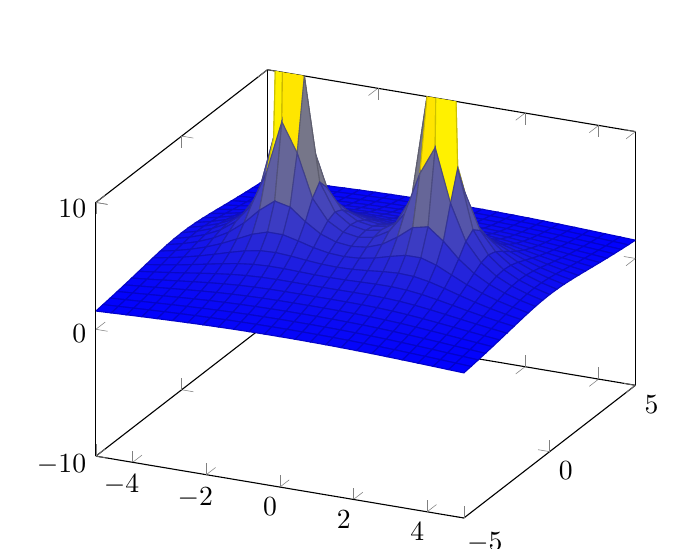
\begin{tikzpicture}
    \begin{axis}[zmin = -10, zmax = 10]
        \addplot3[surf]{5/sqrt(((x+2)^2)+y^2) + 5/sqrt(((x-2)^2)+y^2)};
    \end{axis}
    \end{tikzpicture}
\end{center}

\newpage 

Let's take a look at another example, this time with a positive and a negative charge. The voltage graph looks like this:

\begin{center}
    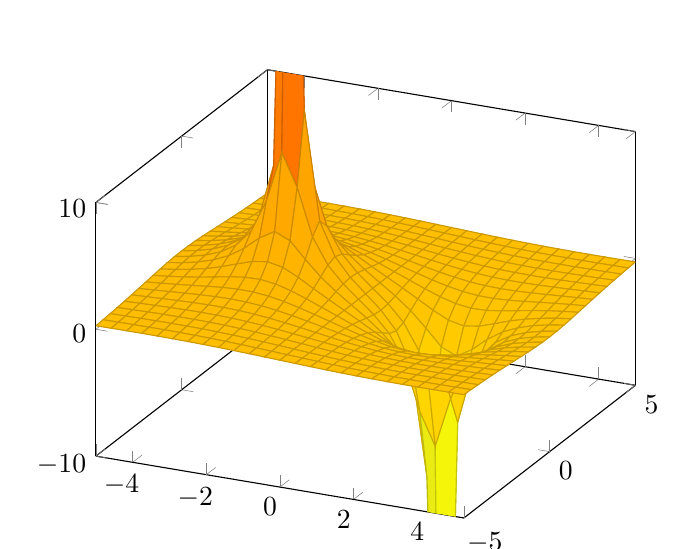
\begin{tikzpicture}
    \begin{axis}[zmin = -10, zmax = 10]
        \addplot3[surf]{5/sqrt(((x+2)^2)+y^2) - 5/sqrt(((x-2)^2)+y^2)};
    \end{axis}
    \end{tikzpicture}
\end{center}

The e-field is no longer zero, but electric potential is zero. Note that this does not mean that a test charge at the midpoint beetween the two charges won't move. It simply means that the the test charge has zero potential energy per unit charge \textit{relative to a chosen reference point} (infinity in this example).

\begin{Problem}
    Rank the four points (A,B,C,D) from largest to smallest magnitude of electric field 
    \begin{center}
        \includegraphics[width=6cm]{Example.png}
    \end{center}

    \tcblower

    \textit{Solution.} When looking at the magnitude of the electric field, we are interested in the slope of the electric potential. Since closer equipotential lines have a greater slope, we can rank the four points based on the distance between adjacent lines. 
    \[A > B \approx D > C\]
\end{Problem}

\subsection*{Electric Potential and Voltage}

Voltage is simply the difference in electric potential:

\[\Delta V = V_f - V_0\]

Be careful when talking about electric potential and voltage; they are not the same thing.

\section*{Topic 9.3 - Conservation of Electric Energy}

Recall that the total mechancal energy of a closed, isolated system is given 
\begin{equation*}
    E_{mech} = U + K
\end{equation*}
If energy is conserved, then the change in potential energy and the change in kinetic energy must add to 0. 
\begin{equation*}
    \begin{split}
        \Delta E_{mech} &= 0 \\
        \Delta K + \Delta U &= 0 \\
        \Delta K &= -\Delta U
    \end{split}
\end{equation*}

The potential difference between two points is related to the change in electric potential energy:
\begin{equation*}
    U_E = q\Delta V
\end{equation*}

\begin{Problem}
    An ion with charge $+e$ and mass $m$ has an initial speed $v_0$. The ion accelerates as it moves through a potential difference $-\Delta V$. What is the ion’s final speed?

    \tcblower

    \textit{Solution. }Initially, the particle has only a kinetic energy $KE = \frac{1}{2}mv_0^2$. After moving through the potential difference, the electric potential decreases by $U_E = q\Delta V \Rightarrow e\Delta V$ Our conservation of energy equation is thus:
    \begin{equation*}
        \begin{split}
            \frac{1}{2}mv_f^2-e\Delta V & =\frac{1}{2}mv_0^2 \\
            \frac{1}{2}mv_f^2 & =\frac{1}{2}mv_0^2 + e\Delta V
        \end{split}
    \end{equation*}
    Rearranging to solve for $v_f$,
    \begin{equation*}
        v_f= \sqrt{v_0^2+\frac{2e\Delta V}{m}}
    \end{equation*}
\end{Problem}

\end{document}
